\section{单点定位基本原理}

\begin{frame}{距离与位置}
    \begin{itemize}[<+-| alert@+>] % 当然,除了alert,手动在里面插 \pause 也行
        \item 信号发射点的位置
        \item 信号接收点与信号发射点的距离
        \item[]
        \begin{figure}
            \centering
            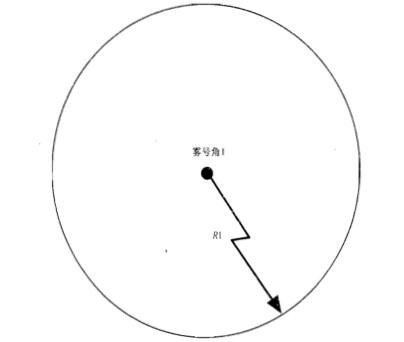
\includegraphics[width=.5\textwidth]{pic/signal_distance.jpg}
            \caption{信号接收点位置分布}
            \label{fig:sig_distance}
        \end{figure}
    \end{itemize}
\end{frame}

\begin{frame}{确定信号接收点位置}
    \begin{itemize}
        \item \textcolor{red}{三个}信号发射点的位置
        \item 信号接收点与信号发射点的距离
        \item[]
        \begin{figure}
            \centering
            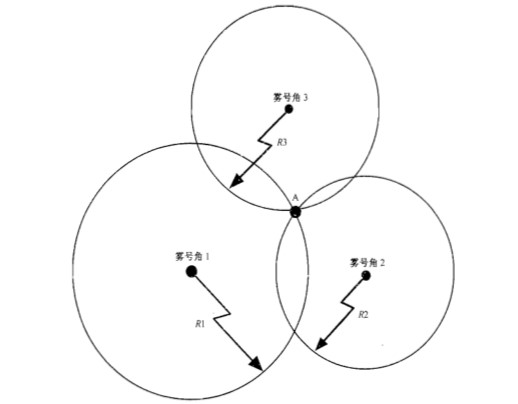
\includegraphics[width=.5\textwidth]{pic/signal_distance_3.jpg}
            \caption{信号接收点位置确定}
            \label{fig:sig_distance_3}
        \end{figure}
    \end{itemize}
\end{frame}

\begin{frame}{信号接收点空间位置确定}
    \begin{itemize}
        \item 接收点$A$坐标 $\left( x _ A, y _ A, z _ A \right)$ \pause
        \item 三个信号发射点$S _ 1, S _ 2, S _ 3$坐标
        $\left( x _ S ^ i, y _ S ^ i, z _ S ^ i \right), i = 1, 2, 3$ \pause
        \item 距离$\rho _ i$为光速$c$与信号传播$\tau _ i$时间的乘积
        \item $A$与$S _ i$距离$\rho _ i$
        \begin{align*}
            \sqrt{ \left( x _ A - x _ S ^ 1 \right) ^ 2 
            + \left( y _ A - y _ S ^ 1 \right) ^ 2 
            + \left( z _ A - z _ S ^ 1 \right) ^ 2 } &= \rho _ 1 \\
            \sqrt{ \left( x _ A - x _ S ^ 2 \right) ^ 2 
            + \left( y _ A - y _ S ^ 2 \right) ^ 2 
            + \left( z _ A - z _ S ^ 2 \right) ^ 2 } &= \rho _ 2 \\
            \sqrt{ \left( x _ A - x _ S ^ 3 \right) ^ 2 
            + \left( y _ A - y _ S ^ 3 \right) ^ 2 
            + \left( z _ A - z _ S ^ 3 \right) ^ 2 } &= \rho _ 3
        \end{align*}
    \end{itemize}
\end{frame}

\begin{frame}{钟差}
    \begin{itemize}
        \item 信号接收点与信号发射点时间\textcolor{red}{不同步}, 时间差异
        称为\textcolor{red}{钟差$\delta _ t ^ A $}, 通常为\textbf{\textcolor{red}{未知量}}\pause
        \item 修正的位置方程
        \begin{align*}
            \sqrt{ \left( x _ A - x _ S ^ i \right) ^ 2 
            + \left( y _ A - y _ S ^ i \right) ^ 2 
            + \left( z _ A - z _ S ^ i \right) ^ 2 } + c \delta _ t ^ A &= \tilde \rho _ 1
        \end{align*}
        未知量$\left[ x _ A, y _ A, z _ A, \delta _ t ^ A \right] ^ \top$, 因此至少需要
        \textcolor{red}{四个}信号发射点信息
    \end{itemize}
\end{frame}

\begin{frame}{Remarks}
    \begin{itemize}
        \item[1] 信号发射点$\left( \text{\textcolor{red}{卫星}} \right)$的位置
        \item[2] 信号发射点与信号接收点$\left( \text{\textcolor{red}{接收机}} \right)$的距离
        \item[3] 求解位置方程获得位置
    \end{itemize}
\end{frame}